\section{Experiment}
We show that \method is a capable and scalable agentic autoresearch framework. 
\begin{itemize}[leftmargin=*, topsep=2pt, itemsep=2pt, parsep=0pt, partopsep=0pt]
    \item \emph{First, \method supports the autonomous policy learning after environment construction. }
    \item \emph{Second, the convergence speed of the success rate \method scales with robot and token resources.}
\end{itemize}
We will focus on the following dexterous tasks, which require precise and reactive control from perceptual feedback: \textbf{Push-T}~\citep{chi2025diffusion}, where the robot uses non-prehensile movement to align a T-shape block to a goal region; \textbf{Pin insertion}, where the robot organizes a pin box by plugging in pins into 4mm-diameter holes; \textbf{GPU-insertion}, where the robot seats GPU chips in thin sockets on the motherboard, and \textbf{Ziptie-cutting}, where the robot grabs and closes scissors to cut the tail of a zip tie. A visualization of these tasks is provided in Fig.~\ref{fig:overview}.

We measure success as the chance of completing a task in one rollout, given a fixed number of retries (here, eight). Unlike measuring success by i.i.d. best-of-N sampling, where each attempt is independent, our retries happen after witnessing the previous failure, implying that our metric captures both precision and in-context recovery in the face of environment uncertainty. We stress that recovery, not just one-shot precision, matters for highly dexterous tasks and reflects the robustness needed for reliable deployment in the real world. 

We use \method to conduct autoresearch in various policy learning paradigms. Coding agents have the freedom to choose various methods and their combinations to solve a task, including end-to-end neural network training such as behavior cloning (BC)~\citep{bc} or real-world reinforcement learning (RL)~\citep{realrl-sac}, as well as gradient-free learning methods such as heuristic learning~\citep{weng2026heuristic} and code-based policy synthesis~\citep{cap}. Our real robot platform is the bimanual 6-DoF YAM robot. We benchmark three coding agents in our physical autoresearch experiments, namely, Codex with GPT-5.5 xhigh~\citep{openai2026codex}, Claude Code with Opus 4.7 High~\citep{anthropic2026claudeopus47}, and Kimi Code with Kimi K2.6 thinking~\citep{moonshot2026kimicode}. 


\subsection{Autoresearch for Heuristic Learning}
\begin{figure}
    \centering
    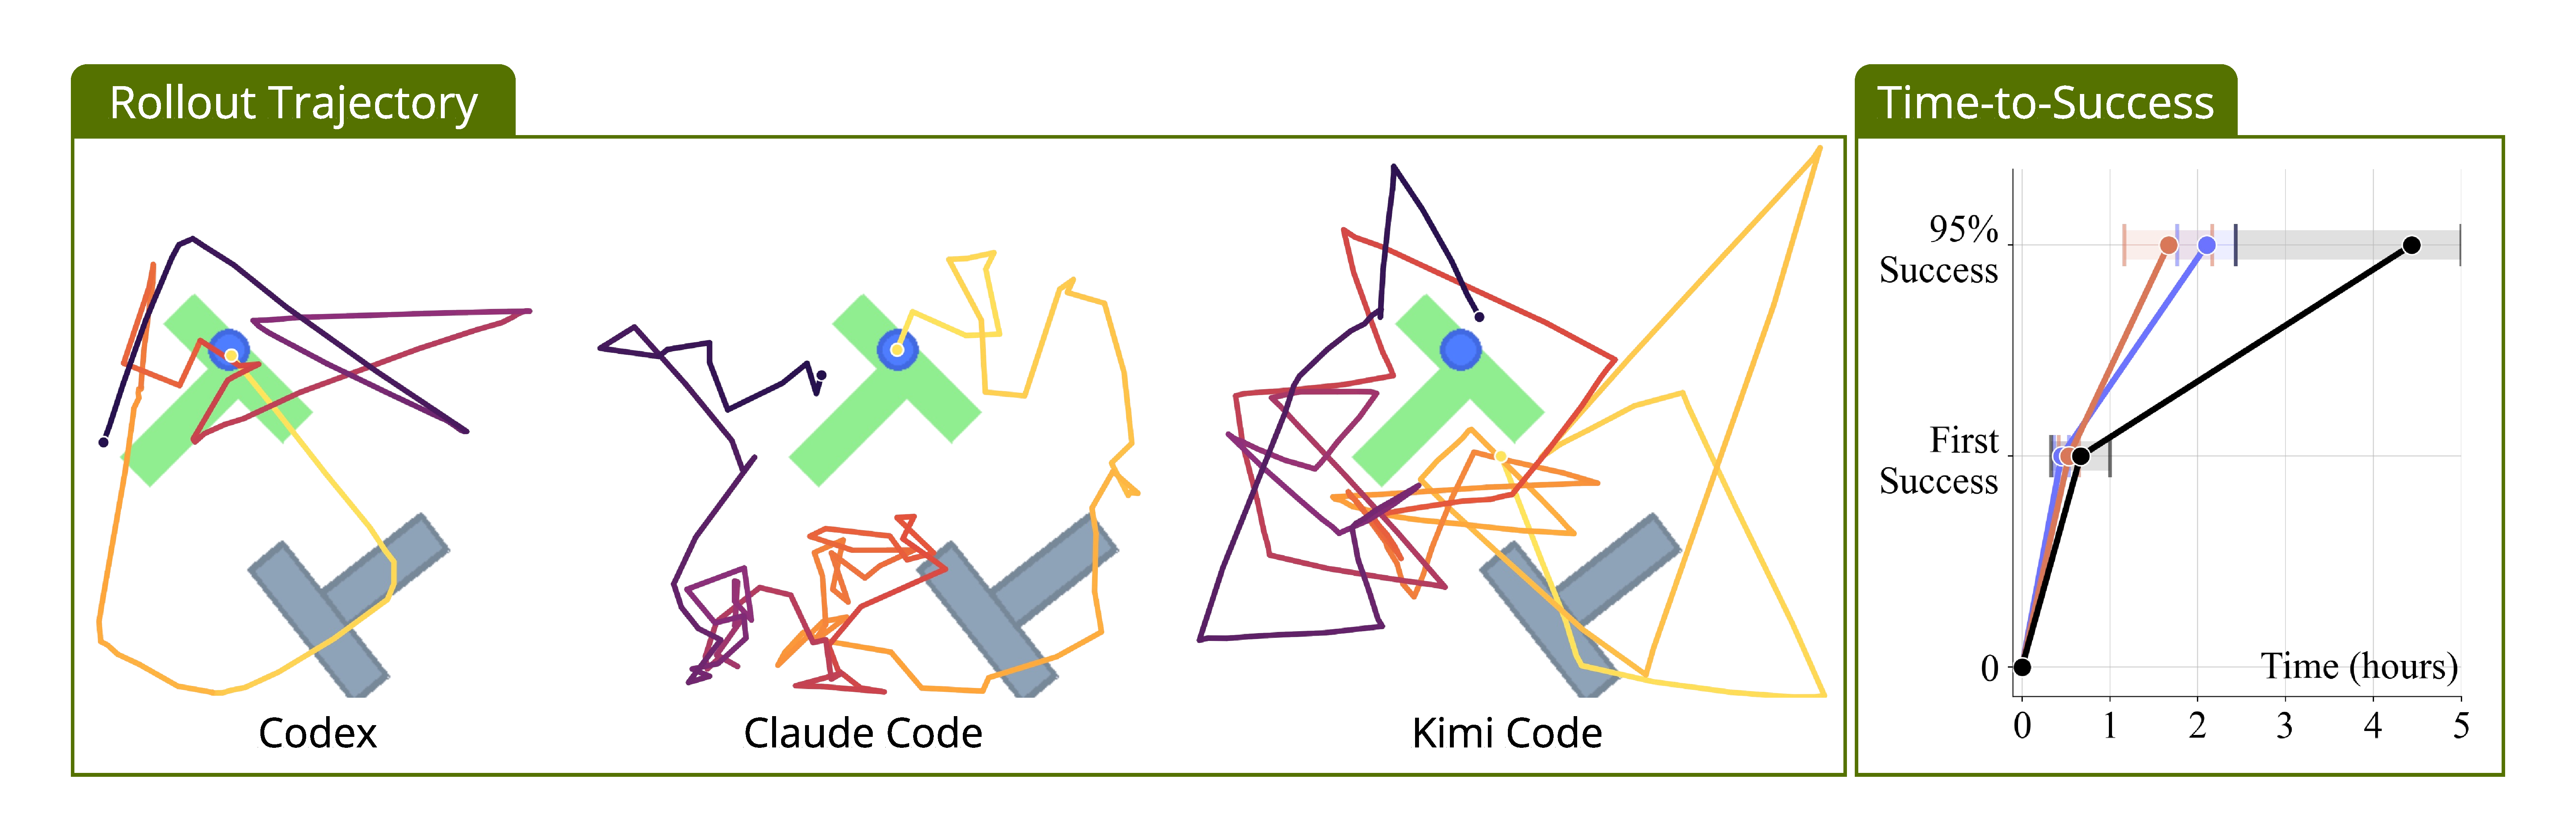
\includegraphics[width=0.9\linewidth]{corl_2026_template_submission/figures/example/gym-pusht.pdf}
    \caption{\textbf{Autonomous heuristic learning in simulation}. On the Gym-PushT~\citep{gympusht} benchmark, Claude Code (orange) and Codex (blue) achieve 95\% success rate within approximately 2 hours, while Kimi Code (black) takes twice the time. 
    } 
    \label{fig:sim_real_pusht}
\end{figure}
We tested \method's ability to drive automatic policy improvement in its simplest form:  learning heuristics~\citep{weng2026heuristic} by synthesizing perception and control tool calls~\citep{cap}. To this end, we built a real-world \textbf{Push-T} environment with its simulation counterpart for comparison. 

\paragraph{The unique challenge of physical autoresearch} As illustrated in Figs. \ref{fig:sim_real_pusht} and \ref{fig:real_pusht_pin_insertion}, all coding agents successfully solve the Push-T task in simulation using heuristic learning. However, the real-world environment proves significantly more challenging, causing two of the three agents to fail. While simulators offer consistent, predictable physics for low-variance hypothesis testing, real-world conditions are non-deterministic and time-varying: factors such as robot dynamics, contact friction, and object movements are inherently less predictable and vary across trials and hardware.

To improve real-world robustness, in subsequent tasks, we encourage agents to explore and even combine diverse learning methods that span heuristics and gradient-based learning, to tackle the corner cases in real-world deployment. We also propose scaling up a physical agent team to test hypotheses in diverse and nondeterministic real-world physics. We will elaborate on these designs in subsequent sections. 

\subsection{Autoresearch for Gradient-Based Policy Improvement}
\label{sec: pin insertion}
Apart from supporting heuristic learning, \method is also capable of training end-to-end policies in a precision-critical task, pin insertion, as shown in Fig.~\ref{fig:real_pusht_pin_insertion}. In this task, coding agents are required to achieve 50 consecutive successes in real-world evaluations. The agents tested multiple methods to improve the policy, including behavior cloning (BC), iterative BC with online rollout data aggregation, and online, offline, and offline-to-online RL with a BC regularization term. The agents also tuned parameters such as batch size, the actor-critic policy update rate, and the BC-term hyperparameters.


% Each run begins from a clean slate: all prior data and checkpoints are removed, and only the 100 human demonstration episodes are retained. For multi-agent teams, we clone a fresh copy of a shared repository for each run and allow agents to commit their contributions back to the origin. In this way, every agent can observe the others' changes, draw on other branches, and decide whether to reuse code or borrow ideas.

% single agent tunnel vision % literture review. 



% The human-supervised environment construction serves as a scaffold that isolates the critical phase during which the agent conducts auto-research. The agent has the freedom to seek algorithm improvements, tune hyperparameters or data formulation, develop code snippets as reusable tools, and/or orchestrate them into a task-oriented program. 
% For the \textbf{Push T} task, we focused on the heuristic learning setting. We provided task context via a text-based description, and the agent can access a visual feedback tool for gripper tip tracking, which was developed alongside the reward in stage 1.
% For the \textbf{Pin Box} task, we first collect 100 successful human demonstrations (on the final insertion stage) and launch real-world RL training using PLD~\citep{pld} to acquire a mediocre policy (approximately 40\% success rate). We provide these 100 demonstrations (approximately), all rollout data generated by the RL training (a few hundred episodes of approximately 0.7h of data), and the checkpoint to warm-start. We instantiate workers with three frontier coding agents -- Codex~\cite{openai2026codex}, Claude Opus 4.7~\citep{anthropic2026claudeopus47}, and Kimi~\citep{moonshot2026kimicode} -- each using its native coding interface, while \method provides the shared task description, goal-oriented documentation, exposed robot APIs, environment interface, and experiment protocol as a harness. We disclose complete experimental details in the Appendix.

% As demonstrated in \ref{fig:hil-climb}, \method enables frontier coding agents to perform policy improvement on real hardware: given a fixed agent-authored environment and scalar feedback from stage 1, the agent iteratively proposes policy or algorithm variants, evaluates them through budgeted physical rollouts, and uses the resulting feedback to select and refine higher-performing candidates. In \texttt{the pin} insertion task, both Claude and Codex deliver a policy with a near 100\% success rate, while Kimi-CLI is slightly underperforming. 




\subsection{Scaling Policy Learning on a Robot Fleet}
We further study whether scaling the number of robots and agents reduces the wall-clock time required to achieve the same target task performance. We assign one coding agent to one robot, and set up identical environment interfaces, reward functions, and reset mechanisms on this robot fleet. We consider fleet sizes of 1, 4, and 8 robots in Push-T and pin insertion tasks. 

In Push-T, scaling from one to eight agents reduces the time to reach a 1.0 normalized score from roughly five to two hours. In pin insertion, scaling from one to eight agents reduces the time to reach a near-perfect success rate from more than 1.5 hours to approximately 40 minutes.
This shows that \method is capable of transferring additional robot resources to faster policy improvement through distributed hypothesis selection. 

% We observe that the fleet is spontaneously coordinated without a centralized scheduler. Each agent works on its own branch of a shared GitHub repository, commits code and results, and can inspect peer branches, experiment logs, and dialogue traces before selecting its next hypotheses. In practice, this produces self-driven collaboration: agents reuse successful implementations, avoid hypotheses already falsified by peers, and redirect their own search based on evidence produced elsewhere in the fleet. Thus, the scaling result is not simply parallel execution of independent trials; it shows that a lightweight version-controlled research substrate is sufficient for multiple coding agents to coordinate the physical policy search. Overall, these results suggest that the \method harness supports fleet-scale physical auto-research: adding robot--agent workers reduces wall-clock search time while preserving the same environment-driven policy-improvement loop used in the single-agent setting. 

% and Autonomous Domain Randomization:
In a multiagent setting, \method can also leverage code-based policies to automatically apply domain randomization during reset. For example, the variations in spatial configurations during GPU insertion span a significantly broader range than prior work~\citep{pld}, which enforces stronger policy robustness. 


% We study whether increasing the number of robot-agent workers reduces the wall-clock time required to reach the same task performance. We consider Push-T and pin insertion, using the same environment interfaces, scoring functions, and reset mechanisms as in the single-agent experiments that are established in stage one. Each worker consists of one physical robot setup and one coding agent session.

% The objective is to measure whether autonomous physical research throughput improves as additional hardware and agent sessions are made available. We therefore compare fleet sizes from one to four robots and track the time required to discover a policy or heuristic that reaches the target task score. On Push-T, scaling from one robot to four robots substantially reduces the effective iteration time: the four-robot fleet reaches a score of $1.0$ in approximately one hour, whereas the single-robot setting requires roughly four hours of exploration to reach the same score. This trend indicates that \method can convert additional physical resources into faster best-so-far policy improvement, provided that candidate evaluations can be distributed across workers. We are currently extending the same protocol to an eight-robot fleet, where we expect further reductions in time-to-score but also larger coordination overhead.

% We observe that the fleet is spontaneously coordinated without a centralized scheduler. Each agent works on its own branch of a shared GitHub repository, commits code and results, and can inspect peer branches, experiment logs, and dialogue traces before selecting its next hypotheses. In practice, this produces self-driven collaboration: agents reuse successful implementations, avoid hypotheses already falsified by peers, and redirect their own search based on evidence produced elsewhere in the fleet. Thus, the scaling result is not simply parallel execution of independent trials; it shows that a lightweight version-controlled research substrate is sufficient for multiple coding agents to coordinate the physical policy search. Overall, these results suggest that the \method harness supports fleet-scale physical auto-research: adding robot--agent workers reduces wall-clock search time while preserving the same environment-driven policy-improvement loop used in the single-agent setting. 

% % and Autonomous Domain Randomization:
% Furthermore, leveraging code-based policies, our resetting procedure supports automatic domain randomization during novel tasks~(Fig.~\ref{fig:gpu_insert_dr}). For instance, the variations in spatial configurations during multi-GPU insertion span a significantly broader range than prior work ~\cite{pld}, which enforces stronger policy robustness. 

\begin{figure}
    \centering
    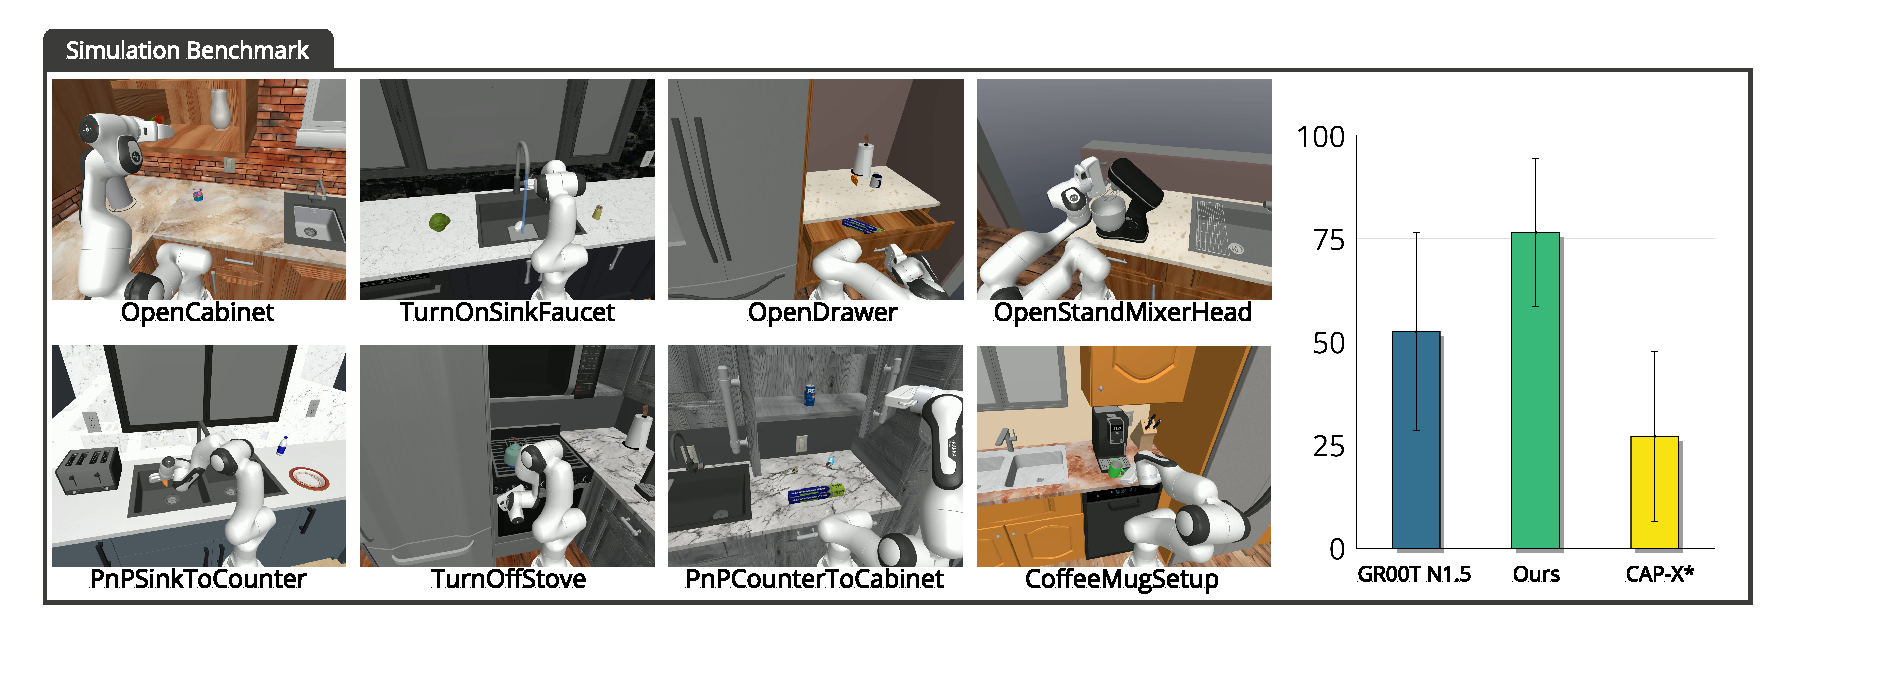
\includegraphics[width=1\linewidth]{corl_2026_template_submission/figures/stats/RoboCasa365.pdf}
    \caption{\textbf{Simulation results}. On RoboCasa365~\citep{nasiriany2026robocasa365} benchmark, \method outperforms end-to-end VLA (GR00T~\citep{gr00tN1}) and zero-shot agentic tool use without autoresearch (CaP-X~\citep{capx2026}).}
    \label{fig:placeholder}
\end{figure}


\subsection{Transferring Autoresearch Experience through Agentic Continue Learning} 
We observe that the insights accumulated by multi-agent physical autoresearch are also transferable to similar, novel dexterous tasks. Following the autonomous exploration phase in pin insertion, agents are prompted to document and reflect on the evolution of their training recipes. When we instantiate a new round of autoresearch for the GPU insertion task, appending this knowledge to the new task's instructions allows coding agents to achieve a high success rate. A detailed analysis is provided in the Appendix.




\subsection{\method Discovers Synergy between Code-Based Policies and VLAs} 
Beyond end-to-end or heuristic training, \method can automatically integrate vision-language-action models (VLAs)~\citep{rt1} with procedural tool calls for long-horizon manipulation. In the RoboCasa365 simulator~\citep{nasiriany2026robocasa365}, the agent boosted the success rate of the GR00T VLA~\citep{gr00tN1} by using motion planning and detection tools to hover above an object before grasping. We successfully transferred this strategy to the real world, where the agent learned to hover over scissors, grasp them, and cut a zip tie, as shown in~\Cref{fig:overview}.



\subsection{Quantifying Agent Resource Utilization}
% MRU, GPU utilization
\begin{figure}
    \centering
    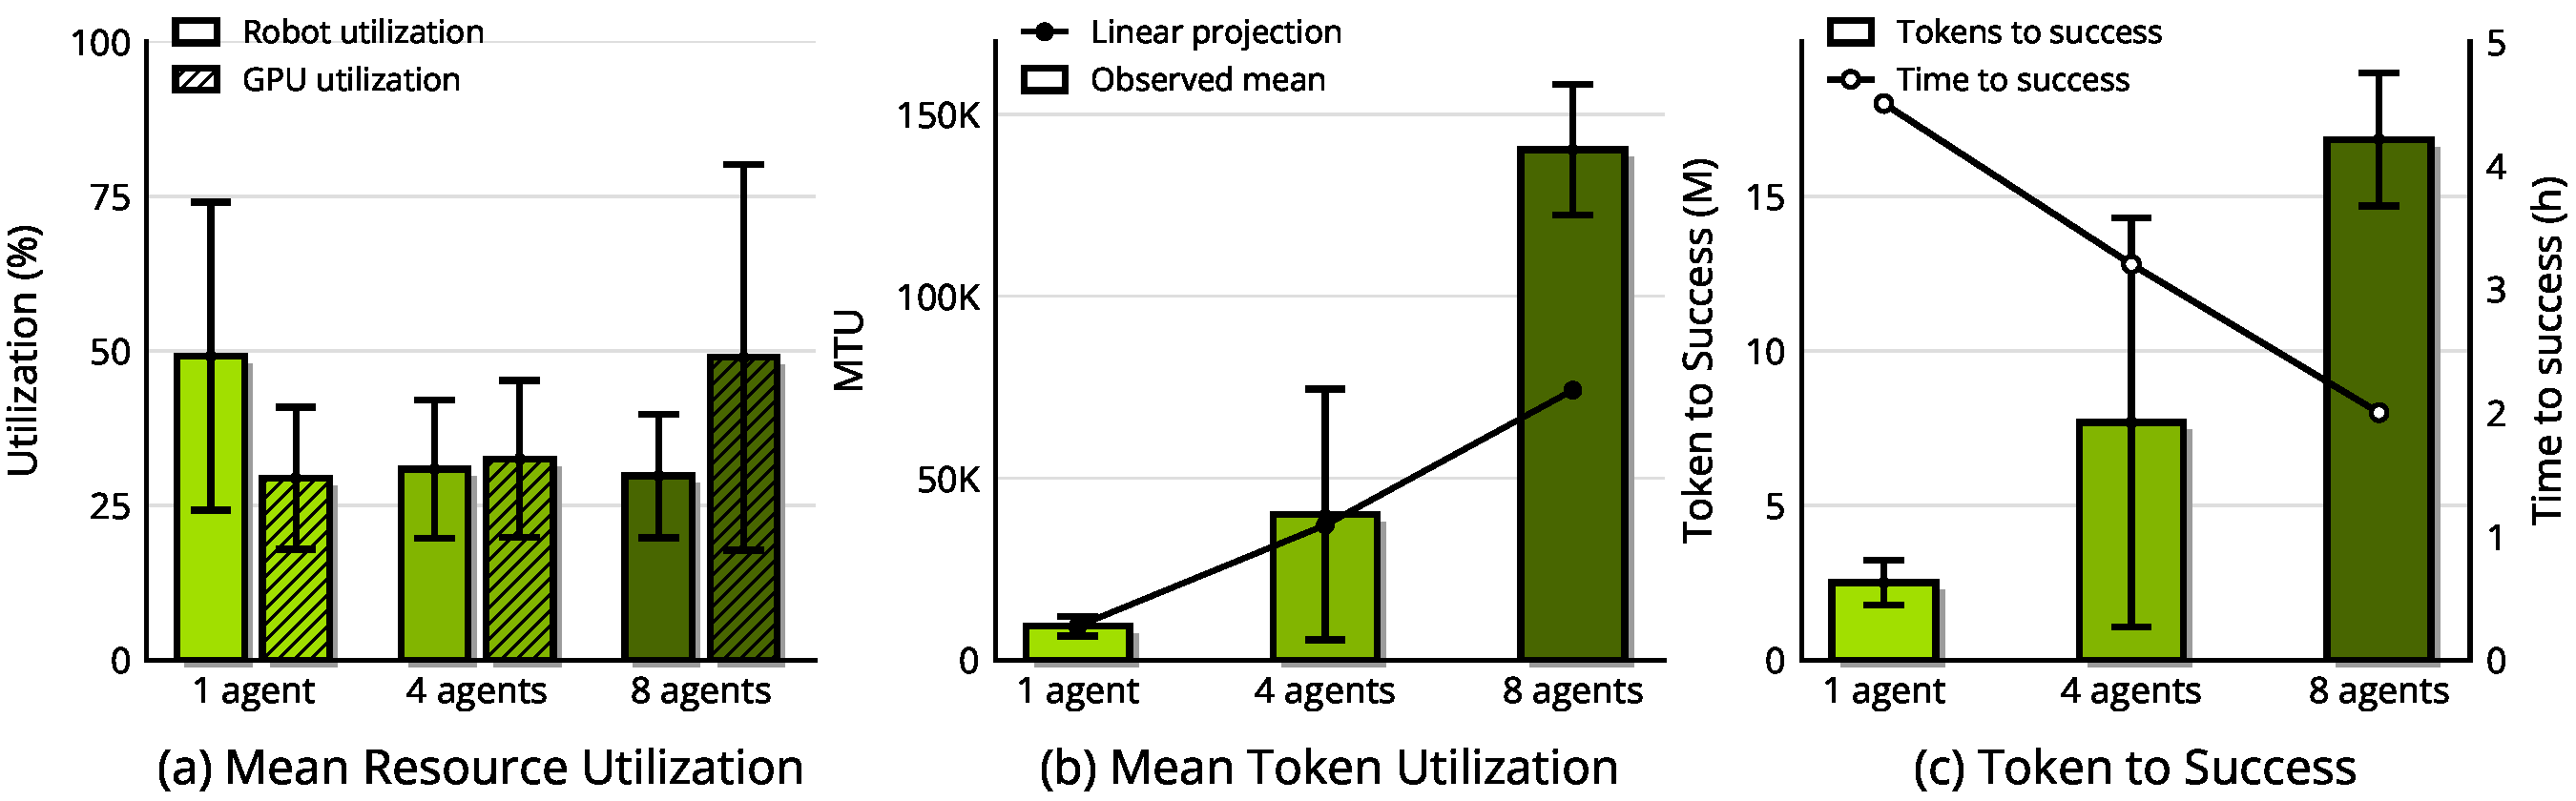
\includegraphics[width=1\linewidth]{corl_2026_template_submission/figures/agent_resource_utilization.pdf}
    \caption{\textbf{Quantifying agent resource utilization}. Scaling from 1 to 8 agents raises GPU utilization and token consumption but lowers per-robot utilization.}
    \label{fig:utilization}
\end{figure}

% save log for Input/output/cache token

\Cref{fig:utilization} summarizes the resource-scaling behavior of ENPIRE on the pin insertion task across single-, four-, and eight-agent fleets. We report Mean Robot Utilization (MRU) and GPU utilization using the definitions introduced above. In addition, we measure Mean Token Utilization (MTU), defined as the number of tokens consumed per minute. We further measure Tokens to Success and Time to Success, which quantify the token budget and wall-clock time required to complete the autoresearch objective.



% To better illustrate the distinction between auto-research on a real robot and in the digital world, we further present results on \texttt{Gym-PustT}. 
% Unlike the real-world setting, the simulation environment provides perfect and closed-form dynamics with no controller error and accurate feedback. Meanwhile, reset and reward are trivially presented. We observe that Codex matches Claude's performance in simulation but underperforms Claude in the real world. On closer inspection, both Claude and Kimi put in a great deal of effort to figure out the dynamics gap...
% \footnote{Although policy research can be initiated in simulation and subsequently transferred, dexterous tasks exhibiting high sensitivity to physical dynamics still necessitate an autonomous, real-world verification loop. } 



% \begin{figure}
%     \centering
%     \includegraphics[width=1\linewidth]{corl_2026_template_submission//figures//placeholder/rl-demo.pdf}
%     \caption{Enter Caption}
%     \label{fig:placeholder}
% \end{figure}

% \begin{tcolorbox}
% \red{
% 1. sim PushT v.s. real PushT: sim works does not mean real works, motivate necessity of real-world policy improvement\\
% 2. PushT: gradient-free (heuristic) learning made possible.\\
% 3. Pin insertion: BC/RL policy improvement made possible.  \\
% 3+. Scaling up Pin insertion to agent teams accelerates search \\
% 4. GPU/Ziptie insertion: continual learning allows transferring knowledge of the training recipe across tasks. 
% }
% \end{tcolorbox}

% Why do we need real instead of sim, and why need multiagents to combact statistical uncertainty. 




% We mainly consider the following manipulation tasks in the real world; task visualization can be found \ref{fig:teaser frame}: 1) \textbf{Push T.} We modify the original push-T task~\citep{chi2025diffusion} task: The robot must push the T block from a fixed initial pose to a fixed goal pose via 2d movement. We set 4 milestones (making contact with the T block, pushing it close to the goal's xy position, aligning it with the goal in orientation, aligning with the goal in both xy position and orientation) as the feedback to simplify credit assignment. 2) \textbf{Organizing Pin Box} Pick up the pin (4mm diameter) from the table and insert it into the hole in the pin box. This task requires the robot to first adjust the pin to align with the gripper tip, preparing for insertion. The pinhole is difficult to discern visually, and insertion requires millimeter precision.


% In this section, we study the extent to which our framework is capable of, by answering the following questions: 1) Can \method framework enable autonomous policy improvement? 2) Can \method framework enable performance to scale with resources (robot, compute, and agent)? 3) Can \method conduct meaningful algorithm research for real-world RL?  

  % \item \textbf{Zip Tie Fastening.} The robot needs to thread a zip tie tail through its narrow locking slot. This task involves high-precision control of a deformable object with tight tolerances. 

% In addition, we provide results of two simulation benchmarks: 1) \textbf{Gym-PushT}: a light-weight 2-d gymnasium environment from the original \texttt{Push T} challenge; 2) \textbf{Robocasa365}~\citep{nasiriany2026robocasa365}: A large-scale simulation benchmark built on the RoboCasa platform, containing comprehensive everyday mobile manipulation tasks across 2,500 diverse kitchen environments. 

% Teaser frames (pushT + pin)


% We examine our framework's capability to perform policy improvement via unattended auto-research on a pair of 7-DoF YAM robot arms developed by I2RT~\cite{i2rt_yam_arm}. With a single objective to deliver a performant policy, the agent can seek solutions under different searching and learning paradigms: 1) Heuristic Learning~\citep{weng2026heuristic} (HL, gradient-free in-context learning): Coding agent updates a heuristic code as policy based on environmental feedback; 2) Deep Learning (DL, gradient-based learning): Coding agent improves an end-to-end neural network policy by iteratively launching real-world evaluation or data collection, the policy can be either trained online via reinforcement learning or offline via behavior clone or both. 
